\chapter{Clusters of the Hdr Image Dataset}
\label{app:clusters}

\begin{figure}[h!]
\begin{center}
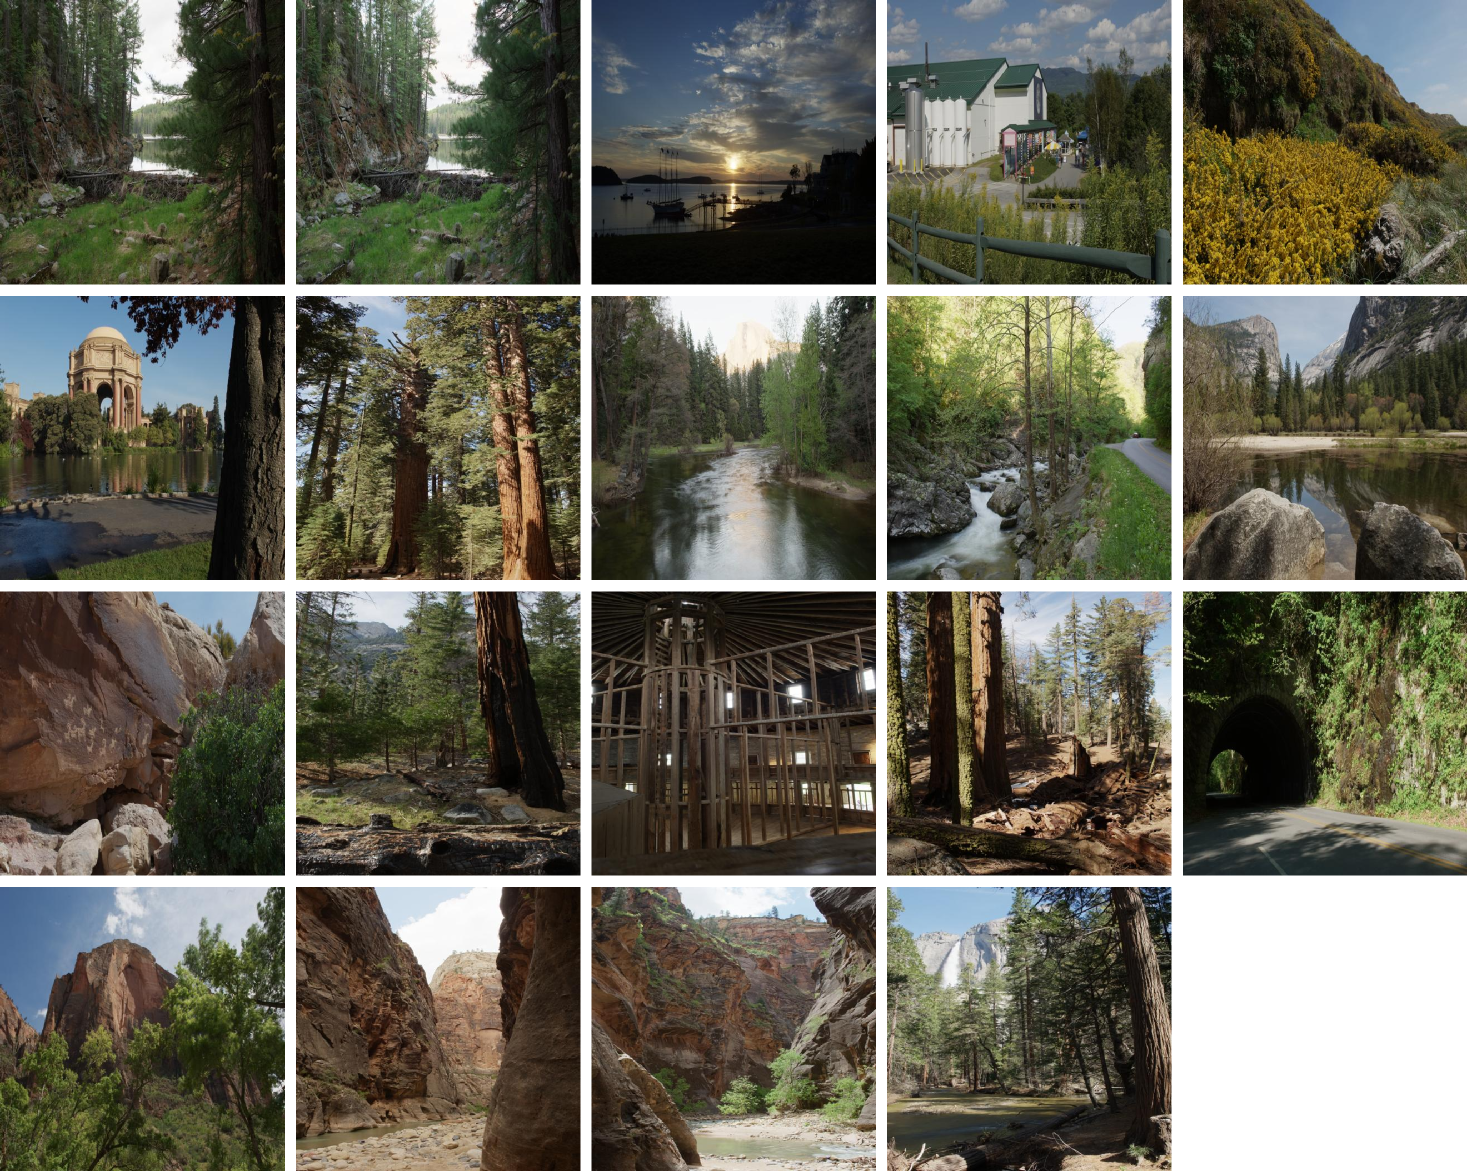
\includegraphics[width=\textwidth]{appendix1/cluster1.png}
\caption{Cluster I, clustering result of Fairchild's HDR Dataset~\cite{fairchild2007hdr} for calibration image selection.}
\end{center}
\end{figure}

\begin{figure}
\begin{center}
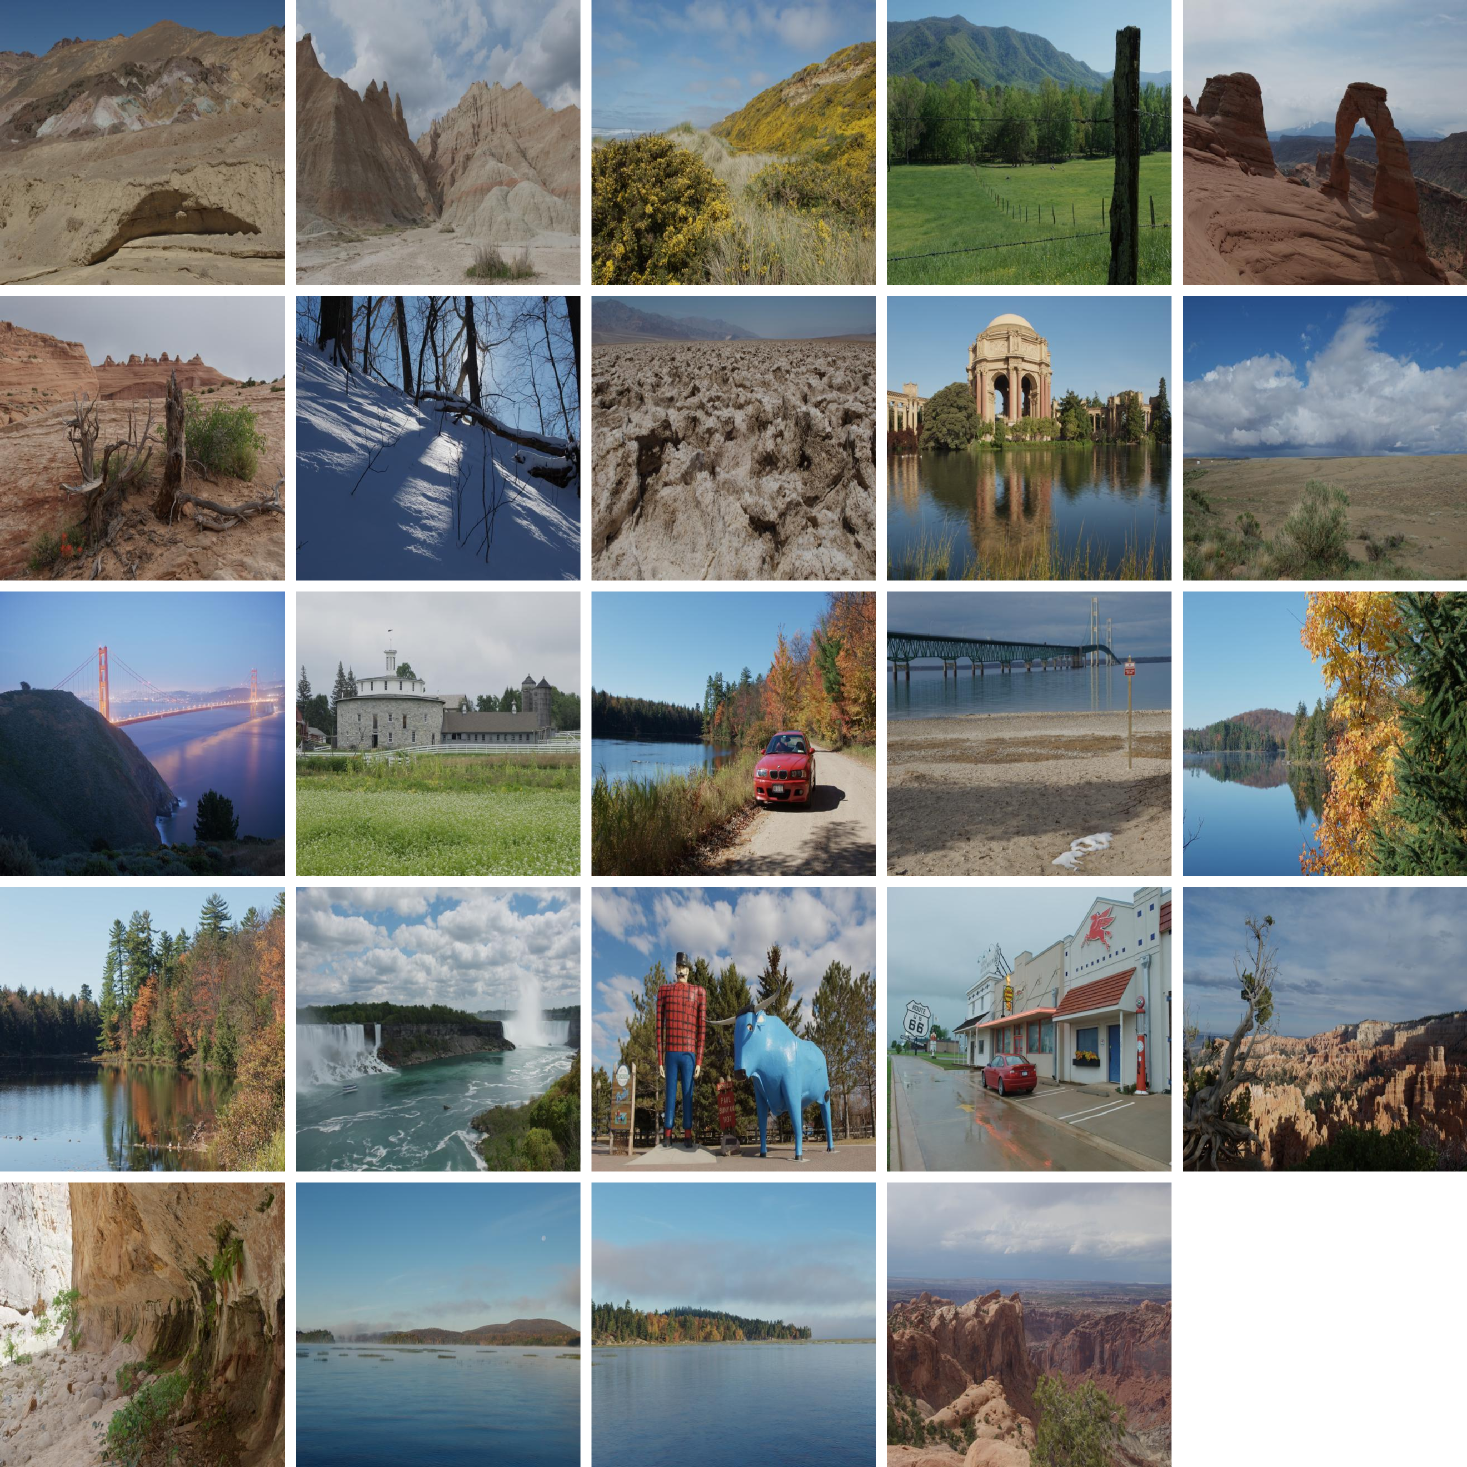
\includegraphics[width=\textwidth]{appendix1/cluster2.png}
\caption{Cluster II, clustering result of Fairchild's HDR Dataset~\cite{fairchild2007hdr} for calibration image selection.}
\end{center}
\end{figure}

\begin{figure}
\begin{center}
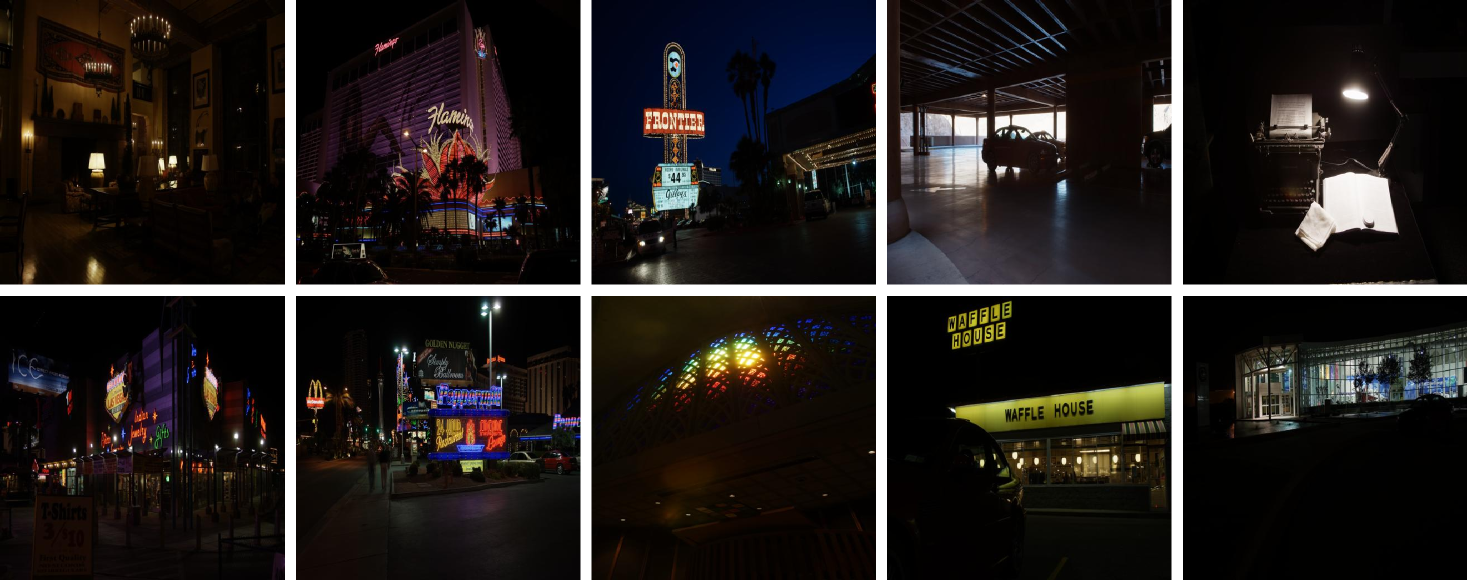
\includegraphics[width=\textwidth]{appendix1/cluster3.png}
\caption{Cluster III, clustering result of Fairchild's HDR Dataset~\cite{fairchild2007hdr} for calibration image selection.}
\end{center}
\end{figure}

\begin{figure}
\begin{center}
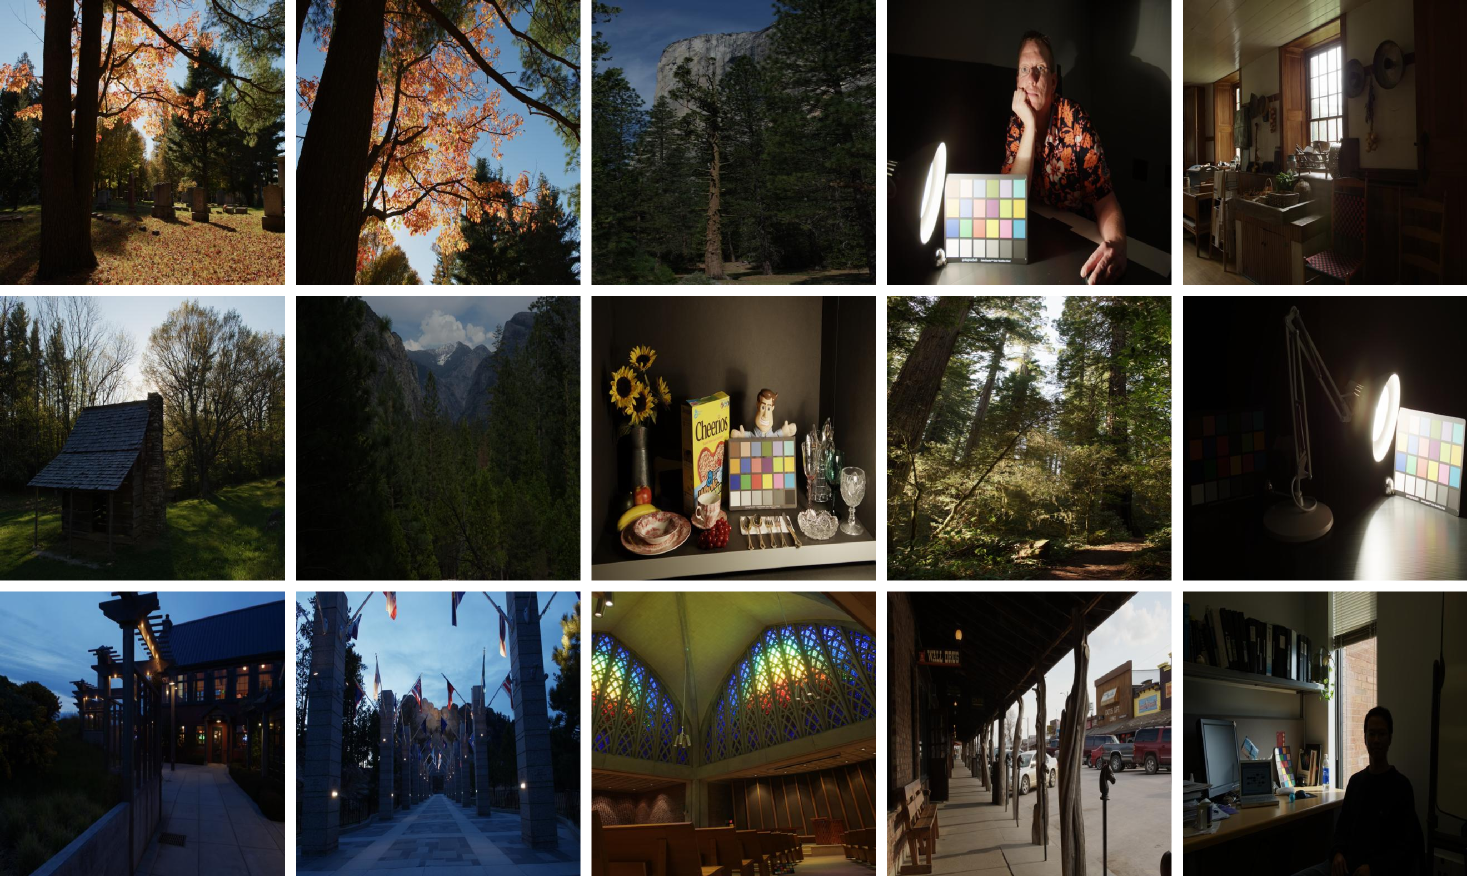
\includegraphics[width=\textwidth]{appendix1/cluster4.png}
\caption{Cluster IV, clustering result of Fairchild's HDR Dataset~\cite{fairchild2007hdr} for calibration image selection.}
\end{center}
\end{figure}

\begin{figure}
\begin{center}
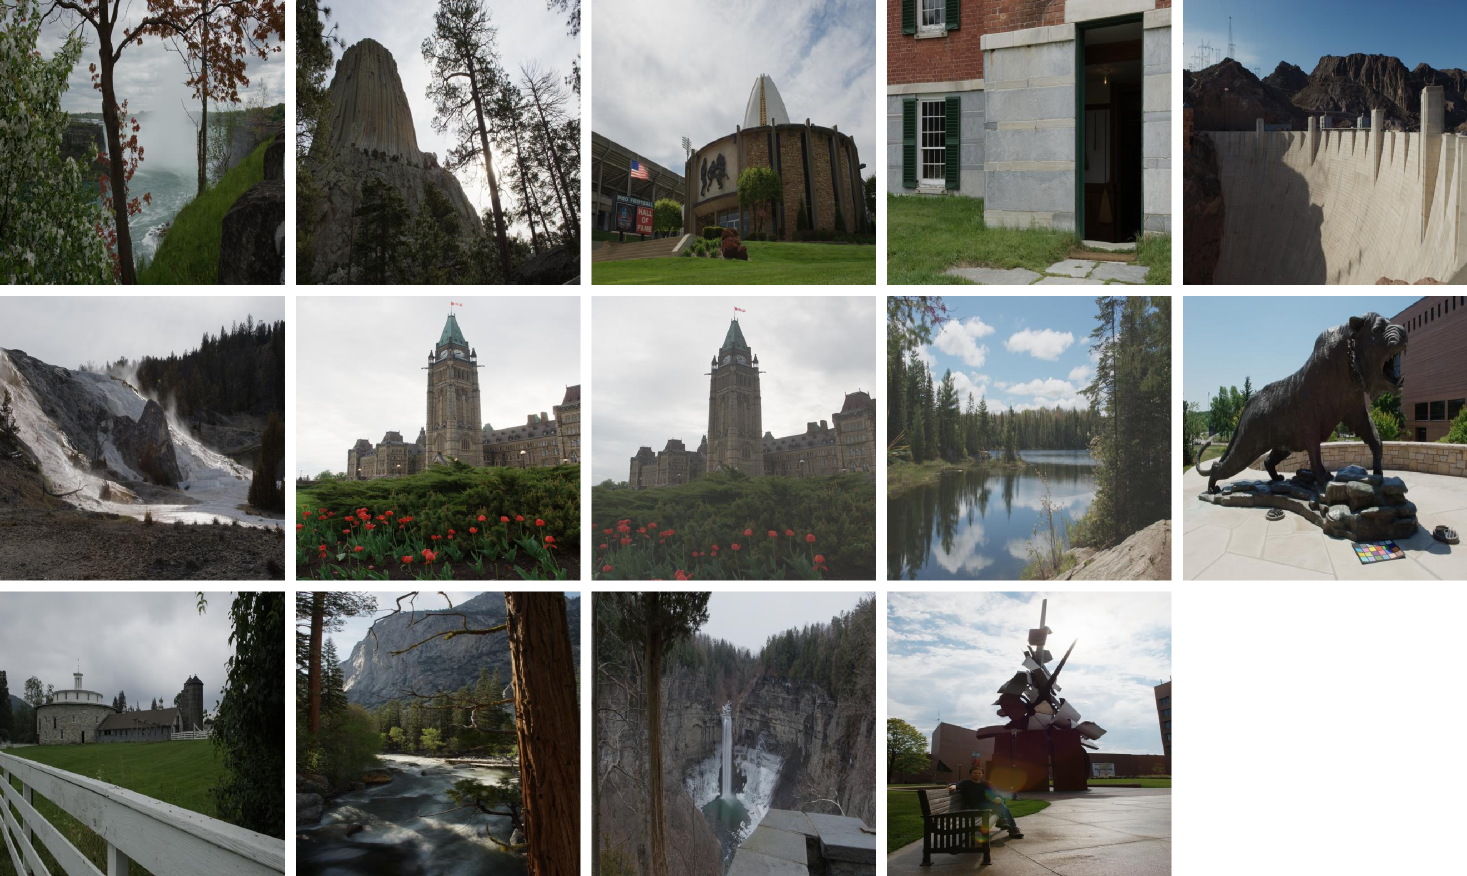
\includegraphics[width=\textwidth]{appendix1/cluster5.png}
\caption{Cluster V, clustering result of Fairchild's HDR Dataset~\cite{fairchild2007hdr} for calibration image selection.}
\end{center}
\end{figure}

\begin{figure}
\begin{center}
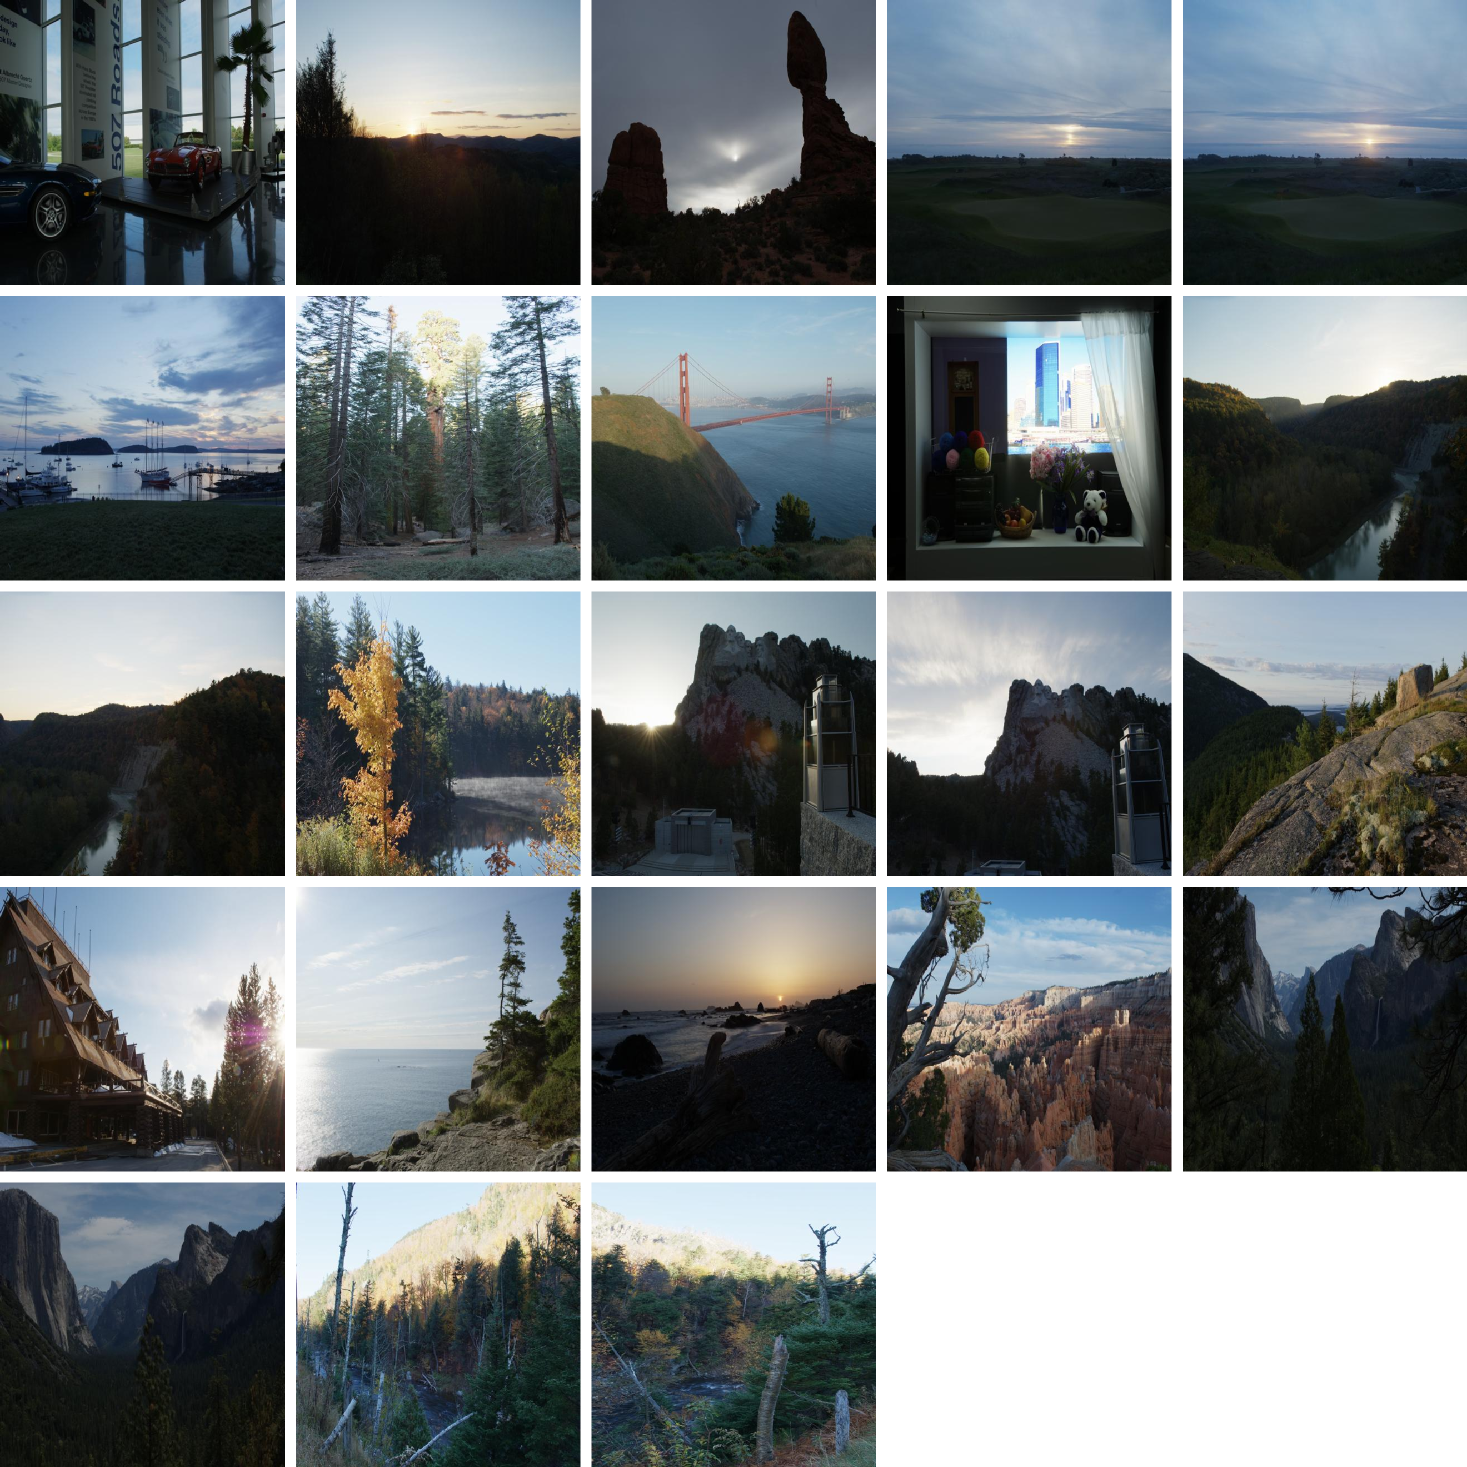
\includegraphics[width=\textwidth]{appendix1/cluster6.png}
\caption{Cluster VI, clustering result of Fairchild's HDR Dataset~\cite{fairchild2007hdr} for calibration image selection.}
\end{center}
\end{figure}